\chapter{Release 2}


\section{Introduction}

Dans ce chapitre, il s'agit d'un release qui consiste en un seul sprint qui est la consultation des rapports ,
afin de pouvoir repr\'{e}senter ces rapports ,nous avons besoins d'abord de determiner
les axes de notre \'{e}tude d\'{e}cisonnelle , puis nous allons \'{e}laborer et tester les rapports en utilisant l'outil Power BI
ensuite nous illustrons la partie ETL(Extract Trasform Load) \`{a} l'aide du l'outil Talend,
et nous finissons par la pr\'{e}sentation des rapports obtenues.


\section{ But de l'\'{e}tude d\'{e}cisionnelle }

Notre \'{e}tude d\'{e}cisionnelle portera sur :
\textemdash{} Le co\^{u}t total de chaque projet
\textemdash{} Le co\^{u}t total des projets pour chaque client
\textemdash{} Le co\^{u}t total par cat\'{e}gorie des projets
\textemdash{} La dur\'{e}e totale du chaque projet
\section{ Elaboration des rapports sur Power BI }
\subsubsection{Pr\'{e}paration}
Nous avons besoin d'ajuster quelques champs pour \^{e}tre ad\'{e}quates \`{a} \^{e}tre
exploit\'{e}es . Par exemple dans la table membre on trouve " firstname " et
"lastname" Et on doit les concat\'{e}ner pour dans une hi\'{e}rarchie pour avoir
des rapports lisibles \`{a} propos des membres .




\FloatBarrier
\begin{figure}[H]
\center
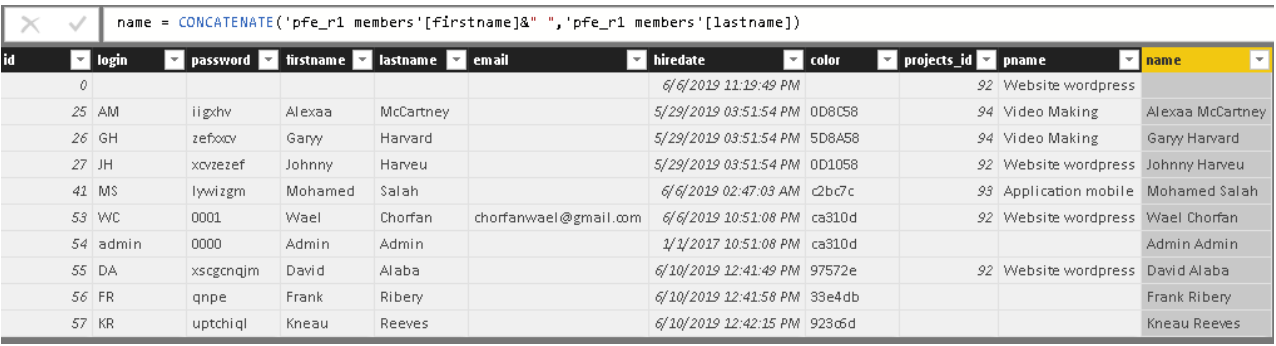
\includegraphics[width=14cm,height=5cm]{./figures/pb1.png}
\caption{Ajustement des noms.}
\end{figure}
\FloatBarrier


\bigskip
\bigskip

\FloatBarrier
\begin{figure}[H]
\center
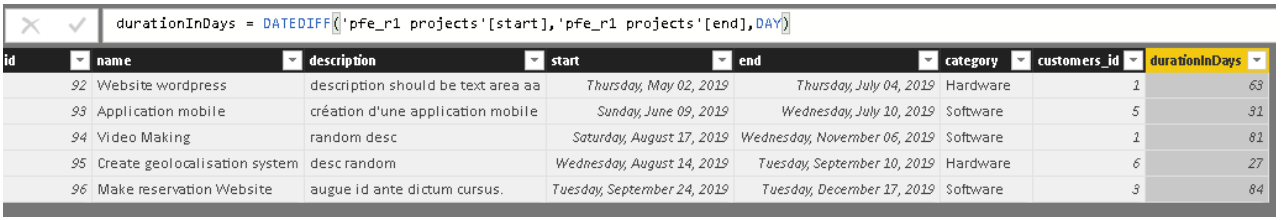
\includegraphics[width=14cm,height=3cm]{./figures/pb2.png}
\caption{Ajustement de la dur\'{e}e totale des projets.}
\end{figure}
\FloatBarrier

\newpage
\subsubsection{Reporting  sur Power BI}
Pour tester les rapports et la validit\'{e} des donn\'{e}es , nous avons utilis\'{e} l'outil
Power BI pour nous donner une impression sur les rapports qu'on doit
int\'{e}grer \`{a} notre application afin de les visulaiser.

\bigskip
Pour ce fait on a cr\'{e}e les rapports correspontdants \`{a} l'\'{e}tude d\'{e}cisionnelle :
Les deux axes importants de l'\'{e}tude sont les couts et la dur\'{e}e :



\begin{itemize}

\item{ \textbf{Les  co\^{u}ts}  }

\FloatBarrier
\begin{figure}[H]
\center
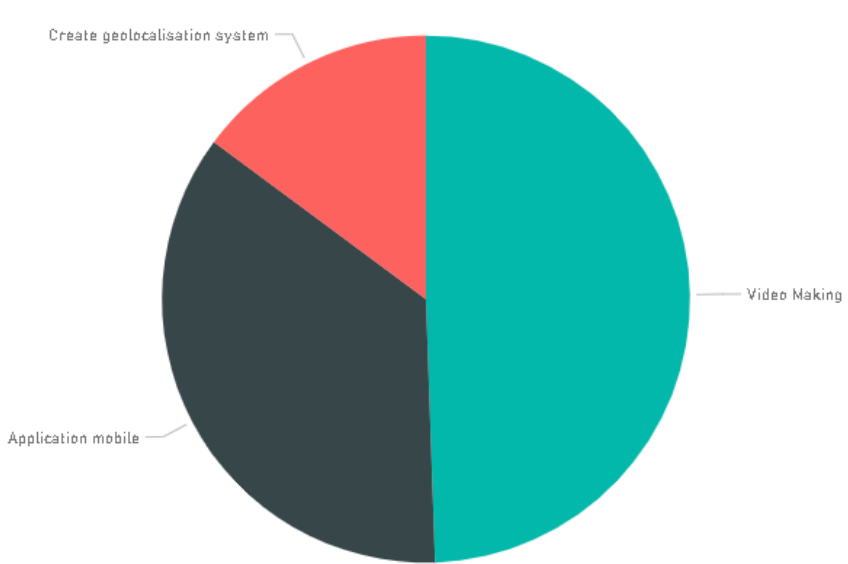
\includegraphics[width=10cm,height=10cm]{./figures/rpb1.png}
\caption{Co\^{u}t total par projet.}

\end{figure}
\FloatBarrier

\FloatBarrier
\begin{figure}[H]
\center
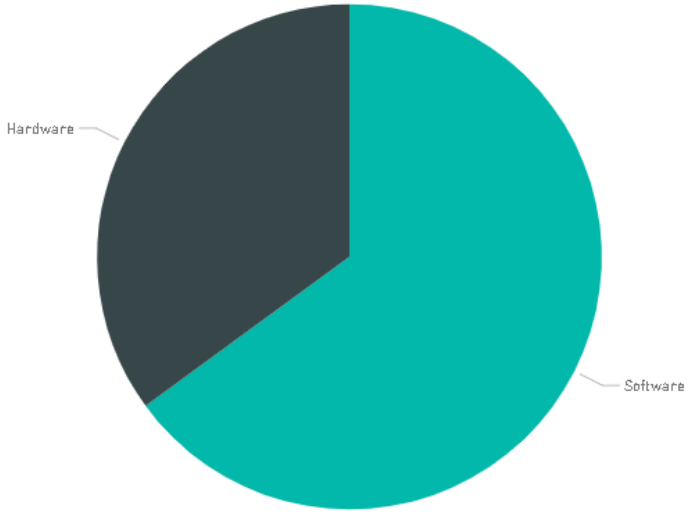
\includegraphics[width=10cm,height=10cm]{./figures/rpb2.png}
\caption{Co\^{u}t total par catégorie de projet.}

\end{figure}
\FloatBarrier

\FloatBarrier
\begin{figure}[H]
\center
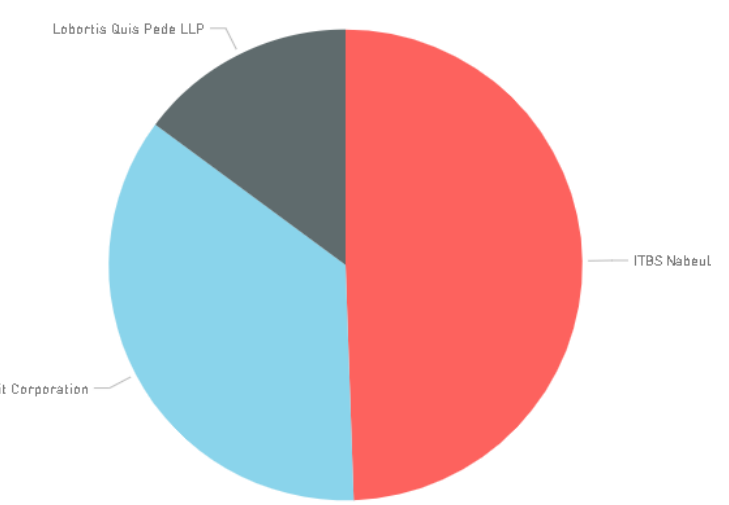
\includegraphics[width=10cm,height=10cm]{./figures/rpb3.png}
\caption{Co\^{u}t total par client.}

\end{figure}
\FloatBarrier

\FloatBarrier
\begin{figure}[H]
\center
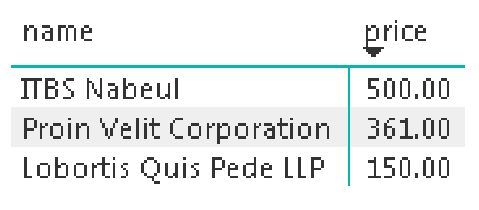
\includegraphics[width=8cm,height=5cm]{./figures/rpb31.png}
\caption{Co\^{u}t total par client en chiffres.}

\end{figure}
\FloatBarrier



\newpage

\item{ \textbf{La dur\'{e}e}  }
\FloatBarrier
\begin{figure}[H]
\center
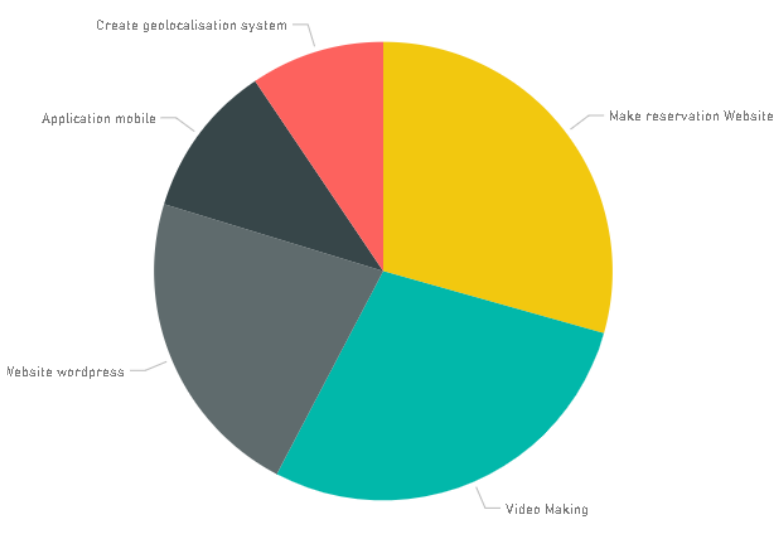
\includegraphics[width=10cm,height=10cm]{./figures/rpb4.png}
\caption{Dur\'{e}e total par projet (en jours).1}

\end{figure}
\FloatBarrier

\FloatBarrier
\begin{figure}[H]
\center
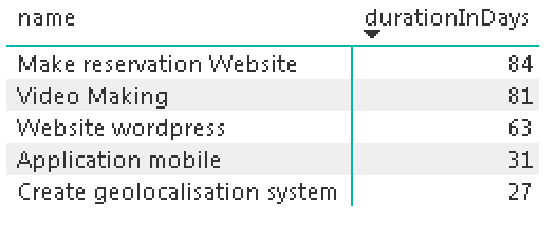
\includegraphics[width=8cm,height=5cm]{./figures/rpb42.png}
\caption{Dur\'{e}e total par projet (en jours).2}

\end{figure}
\FloatBarrier


\end{itemize}




















































\section{ Partie ETL }
Pour avoir des rapports sur l'application web ,on doit avoir les données sous une certaine format ,
afin de satisfaire le besoin de la consultation du suivi des projets selon le temps et le cout.
Ains les données correspondantes sont collectées, modifiées et chargées dans un entrepôt de données
assurant ainsi la phase ETL.

Nous avons utilisé l'outil talend pour charger les données necessaires .
Puisque nous avons les données ordonnées et intégres ,nous n'avons pas été besoin d'une ODS (Operational data source)
nous passont directement à construite notre table de faits

\subsubsection{Analyse}
\subsubsection{Conception}
\subsubsection{Code}
\subsubsection{Test}


